\documentclass{article}
\usepackage[utf8]{inputenc}
\usepackage{courier}
\usepackage[margin=1.0in]{geometry}
\usepackage{hyperref}
\usepackage{listings}
\usepackage{tikz}

\title{Comp 520: Final Project Report}
\author{The Heapsters: Teng Long, Ethan Macdonald, Hardik Vala}
\date{}

\begin{document}

\maketitle

\section{Introduction}

\begin{figure}[h]
  \centering
  
\includegraphics[width=7.5cm]{gopher_python.png}
  \caption{The symbiotic relationship between a Gopher and a Python.}
  \label{fig:gopher-python}
\end{figure}

\noindent This report gives an overview of our GoLite to Python compiler. The compiler source is available here: \href{https://github.com/Sable/comp520-2016-05}{https://github.com/Sable/comp520-2016-05}

\subsection{Motivation}
Our choice to pursue the GoLite project was motivated by the following: First, we wanted to gain insight into the inner-workings of the languages we most frequently use. Most of these are imperative, general purpose languages like GoLite. Secondly, we were more interested in the engineering aspects of the compiler than the design of a domain-specific language. Lastly, we felt that the project might have a bit more structure (i.e., more detailed specifications). We believed this be a good thing since all of us were new to writing compilers and were still developing our intuition with regard to the workload created by various design choices (i.e., we did not want too many degrees of freedom).

We used Java with SableCC3 to build the scanner, parser, and abstract syntax tree (AST) since we had some familiarity with SableCC from the first two assignments, and it simplified much of the heavy lifting for the early stages of the compiler. Thereafter, we utilized the generated SableCC code throughout the rest of the compiler (e.g., for traversing the AST during weeding, type checking, and code generation). This allowed us to focus more the design of our compiler rather than the implementation details. For instance, we were able to focus more on having a correct grammar and well-designed AST in lieu of building our own parser, scanner, and AST from scratch. 

\subsection{Contributions}
\subsubsection{Overall}
Although individual contributions did vary from milestone to milestone, the work was pretty evenly distributed between group members over the course of the semester. When possible, we tried to work in the same physical location with one another. This allowed us to bounce ideas off of each other and sort out complicated issues without miscommunication.

\subsubsection{Milestone \#1}
During milestone 1 Ethan and Leo came up with most of the context-free grammar while Hardik modified it to work with SableCC3 and wrote the semicolon insertion rules, Ethan wrote the report, Leo did the pretty printer, and Hardik did most of the AST. 

\subsubsection{Milestone \#2}
During milestone 2, Ethan and Leo worked on the typechecker and tests together. Ethan wrote the weeder. Hardik wrote the type pretty printer and report. 

\subsubsection{Milestone \#3}
During milestone 3, Hardik re-did the typechecker (everyone agreed it had to be done), Ethan and Leo started redoing the typechecker but passed the task on to Hardik so as not to duplicate work, and Leo did the first part of the code generator. 

\subsubsection{Milestone \#4}
During milestone 4, everyone worked together to finish up the code generator (especially Leo \& Hardik). Ethan wrote the first draft of this report, and everyone made edits as necessary.


\subsection{Resources}
Aside from SableCC3 and Java, the only resources consulted were the reference materials and source code referenced in the README.md of our GitHub repository. Below is another list of hyperlinks to those resources.

\subsubsection{Viewed}
\begin{itemize}
\item \href{https://golang.org/ref/spec}{The Go Programming Language Specification}
\item \href{http://www.sable.mcgill.ca/~hendren/520/2016/tiny/}{Tiny language example}
\item \href{https://github.com/leo-teng-long/minipart2/blob/master/src/mini/PrettyPrinter.java}{Leo's MiniLang Pretty Printer}
\item \href{http://www.sable.mcgill.ca/~hendren/520/2016/joos/jjoos-scc-3/}{JOOS SabelCC 3}
\item \href{http://www.sable.mcgill.ca/listarchives/sablecc-list/msg00639.html}{Re: Redefinition Error}
\end{itemize}

\subsubsection{Used}
\begin{itemize}
\item \href{http://www.sable.mcgill.ca/~hendren/520/2016/semicolon-test/}{Example SableCC code for handling GoLite semicolon rule}
\item \href{http://lists.sablecc.org/pipermail/sablecc-discussion/msg00144.html}{Re: SableCC feature suggestion}
\end{itemize}
\section{Compiler Structure}

In the following sub-sections, we describe each phase of our compiler according to Figure \ref{fig:phase}. (Our compiler doesn't support explicit Resource and Emit phases.)

\begin{figure}[h]
  \centering
  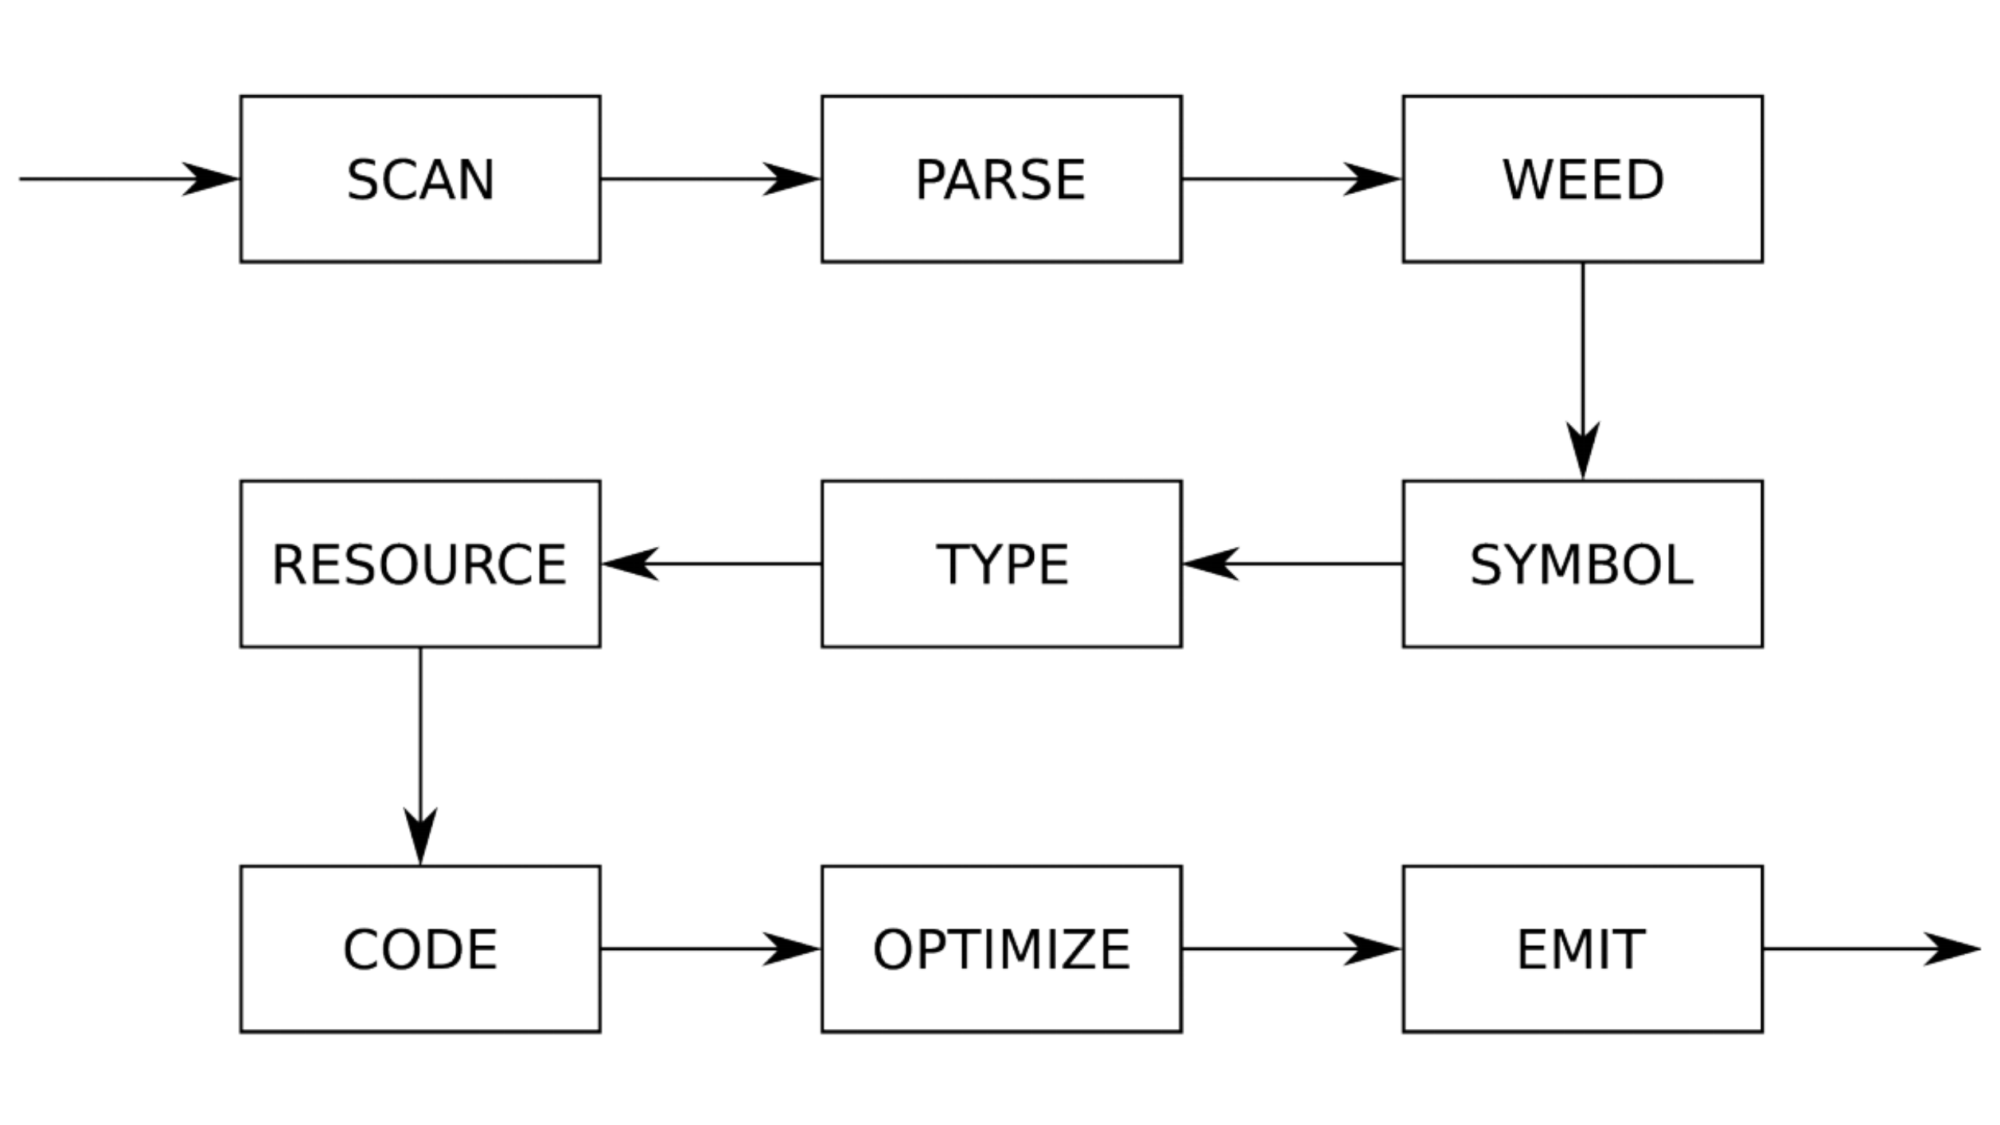
\includegraphics[width=\linewidth]{phase.pdf}
  \caption{Phase diagram.}
  \label{fig:phase}
\end{figure}

\subsection{Scan}

Implementation of the scanner was made fairly straightforward using SableCC3, multi-line comments and optional terminating semi-colons for statements presenting the most challenge. Our regular expression pattern for matching multi-line comments manages to capture most cases, with the exception of edge cases such as \texttt{/**/} between tokens on the same line. Handling optional semi-colons for terminating statements required the use of a semi-colon insertion rule which inserts semi-colons after certain scanner tokens (e.g. right parenthesis), taking special care to properly ignore any intermediate whitespace.


\subsection{Parse}

The parser and AST were also fairly straightforward, it just took a long time to agree upon the precise structure that we eventually went with. The biggest challenge was trying to predict which structures would cause issues during later milestones. During later milestones we wound up going back and modifying our grammar/AST somewhat. Our parser takes in tokens and outputs an AST.

We included constraints within our grammar to reduce the amount of weeding required (e.g., we limited the set of permissible top-level statements). Some issues that we chose to defer until later stages included the removal of quotes/backticks from strings, checking proper usage of breaks and continues, checking that fields and array accesses happen on the correct elements, checking for string casts, checking that expressions in simple\_stmt are valid (e.g., function calls), mismatching numbers of ids and values in declaration statements, and distinguishing between function calls and custom type casts.

Like Go, our parser treats blank tokens, \texttt{\_}, not as regular identifiers, but as ``anonymous" identifiers and ``null" expressions.

\subsection{Weed}

After our milestone 1 was complete we brainstormed a big list of cases that we needed to weed. Later, we thought of a few more weeding conditions while we were working on the typechecker, so we added them. Our weeder takes in an AST and outputs an AST.

Our weeder throws an exception if one of the following occurs:
\begin{itemize}
\item Missing return statement in non-void function (checks all execution paths)
\item Aray in an array access is not non-constant and not a function call
\item Object in a field access is not non-constant and not a function call
\item Type casting for string.
\item Array bound is not an integer
\item Last part of a loop statement is a short assignment
\item Continue statement occurs outside a loop
\item Break statement occurs outside a loop
\item Switch statement contains multiple default cases
\item Decrement is applied to a non-decrementable
\item Increment is applied to a non-incrementable
\item Number of identifiers on the R.H.S. of an assignment, short assignment, or variable specification statement is not equal to the number of expressions on the L.H.S.
\item Expression statement does not comprise solely of a function call
\end{itemize}

\subsection{Symbol \& Type}

Our symbol table is implemented according to the standard approach of using a cactus stack of hash tables, where each table corresponds to a scope and scopes are pushed and popped when entering and exiting scopes, respectively. The symbol table tracks three types of symbols, \textit{variable}, \textit{type alias}, and \textit{function}. As an added challenge, our compiler optionally allows top-level declarations to occur in any order (hence allowing mutually recursive definitions), and is accomplished by performing an extra pass of the program to fill in top-level declarations before proceeding to other declarations.

Our first attempt at this section was quite messy. We made some poor design choices early on. We didn't store enough information in the symbol table (e.g., what kind of symbol). The symbol table just returned the original AST node where the symbol was defined. While this worked alright at first, traversing the tree to get the correct information every time we encountered a symbol turned out too complicated to manage effectively. This was especially challenging for dealing with aliases, which we never got to work in our original implementation. In the second implementation, most of these problems were resolved due to better design. In the second iteration we utilized a better symbol table that kept track of more information, like which kind of symbol. Our typechecker takes in an AST and outputs an AST as well as a type/symbol table.

Our final set of type rules were implemented to conform with Vince's GoLite programs released after Milestone \#2.

\subsection{Code}

We chose Python (2.7) as the target for our compiler for a number of reasons: Python is interpreted rather than compiled, and hence affords the benefits of an interpreted language, e.g. zero time spent compiling. It's well suited for programs with large compile time but a short run time. Moreover, choosing Python as the target allows transmission of compiled output to many remote machines (the output \texttt{.py} file can be run right away, so long as Python 2.7 is installed, which is usually the case for modern machines). The alternative is to transmit the source and compile individually at each remote, as  for many other languages (e.g. C), which can slow down distributed systems. Moreover, we find there is significant overlap between the types of programmers that are attracted to Python and Go, so having a compiler that allows users to convert from one language to the other could prove quite useful (of course, our compiler would require extension to the full language specification of Go). Choosing Python also gave us an opportunity to gain a deeper understanding of static vs. dynamic typing and differing scoping rules, primarily through finding ways to guarantee congruent run-time behaviour between the languages that differ in both these respects. Lastly, the simplicity of Python's language constructs made many aspects of code generation easier to implement. For instance, Python's list and dictionary support proved to be a natural mapping for slices and \texttt{struct} objects, and Python's built-in functions for strings made the handling of string manipulation much easier.

Nevertheless, generating correct Python code that preserved the semantics of GoLite presented a few challenges:
\begin{itemize}
\item The scoping rules for Python are less stringent than GoLite, with functions being essentially the only program element that introduces new scopes. To enforce the scoping rules of GoLite, we implemented an elegant solution that simply renames each symbol according to it's scope depth in GoLite (See the Examples section). This required the use of the symbol table in code generation to track variable and function symbols along with their scope depth.
\item Python permits arbitrarily large integers, where GoLite wraps integers around when they surpass the 32-bit range. To address this, the output of every integer and rune expression is passed to a function that enforces the wrap-around using the following formula,
\begin{equation}
(\mbox{expression} - 2^{31}) \mbox{ mod } 2^{32} - 2^{31}
\end{equation}
(See example 4.2.4 in Examples.) Although this solution properly enforces the correct semantics for integer overflow/underflow, it causes a significant slow down in programs performing numerous arithmetic operations. As a result, applying such normalization is left as a compiler option the programmer must explicitly specify.
\item We used Python while loops in place of Go for loops, because python loops do not map properly to Go for loops (they work more like an iterator than a for loop). (See example 4.2 in Examples.)
\item Python doesn't have switch statements but we found a way to make them work using if/else statements. There are two different cases that need to be considered. The switch statement without expression acts pretty much like an if-else statement, which is fairly easy to implement. The one with expression, however, requires the generated Python code to explicitly compare the values of expressions in switch statement and either case clause. (See example 4.4 in Examples.)
\item Since Python does not allow empty indented block, to handle the cases such as empty functions, we add the keyword \texttt{pass} to the generated code to ensure that a call to an empty function would not raise any errors.
\item An oddity of Python is that functions that reference globally defined variables must be explicitly marked before use in the function (see the Examples section). Our solution involved marking each global variable, obtained from the global scope of the symbol table, inside every function declaration.
\item Because Python abides by the offset rule to indicate blocks and imposes a limit on indentation depth, severely nested structures in GoLite programs, such as chained if-else statements, may produce target programs that crash. Our current implementation of the compiler does not address this and we leave it as a topic for future work.
\end{itemize}

In the design of the code generator, the semantics for certain GoLite elements were non-obvious and hence, we took the liberty of imposing our own semantics:
\begin{itemize}
\item GoLite allows expressions of a non-string base type to be casted to a boolean, and we define the semantics for such castings according to the semantics defined for Python (e.g. Boolean casting a non-zero integer yields true and casting zero yields false).
\item The boolean literals represented by \texttt{true} and \texttt{false} are printed as \texttt{True} and \texttt{False}, respectively.
\item Type alias information is not represented directly in compiled programs, and rather program elements typed by an alias have their types fully resolved before generating the corresponding output. This required the use of the symbol table to access symbols representing type aliases.
\end{itemize}

% \subsubsection{Parser}
% \begin{itemize}
% 	\item Hardik started working bottom-up, and Leo \& Ethan worked top-down on this until we had the entire CFG defined
% \end{itemize}
% \item Figuring out a sensible abstract syntax tree
% \begin{itemize}
% 	\item In later parts of our compiler we wound up having extraneous function calls because of how our AST was defined (e.g., node.getOptId().getId() when, in hindsight, it could have been just node.getId()).
% 	\item Since we're generating Python, it might have been better to have an "elif" statement in our AST, but we didn't realize this until hitting roadblocks during code generation
% \end{itemize}
% \item For the most part this milestone went smoothly (maybe our design choices didn't bother us until later)
% \end{itemize}
% \subsubsection{Weeder}
% \begin{itemize}
% \item Cleaning up cases that we didn't want to handle during parsing (e.g., break/continue statements)
% \item This part was pretty fast to implement/went pretty smoothly
% \end{itemize}
% \subsubsection{Typechecker}
% \begin{itemize}
% \item Made a bad design decision that we paid for dearly later
% 	\begin{itemize}
% 		\item We should have defined our own types
% 		\item We should have defined a symbol class
% 		\item We wound up redoing the entire thing with the symbol class and types later
% 	\end{itemize}
% \item Wound up redoing our typechecker with a more sensible design
% \item Structs and aliases caused us some grief
% 	\begin{itemize}
% 		\item We never did get aliases correct until after we re-did the whole thing
% 		\item Structs were a bit of a pain because we had chosen an AST representation that was more intuitive for writing the AST than it was for writing the typechecker. However, after wrapping our heads around the problem we were able to work around this inconvenience.
% 		\textbf{TODO}: Not true
% 	\end{itemize}

\section{Optimize}

Although optimization is outside the scope of the project, we attempt to
make our generated Python code as efficient as possible. \textit{1)} When
generating code for integer and rune literals in safe mode, we check if
values of the literals are within the range of int32. The normalization 
is only applied to literals that are outside of the range. \textit{2)}
Since appending elements to the same slice is a quite common operation,
we separate it in two different cases when generating the \textit{append}
statement. When the returned slice is caught by the same identifier, we
generate the following code: \textit{list.append(...)} (instead of
\textit{list = list + [...]}), as the later is a slower operation than 
the former.

\section{Examples}

\lstset{frame=tb,
  showstringspaces=false,
  columns=flexible,
  basicstyle={\ttfamily},
  numbers=none,
  breaklines=true,
  breakatwhitespace=true,
  tabsize=3
}

\subsection{Hello World}
\subsubsection{Notes}
Basic ``Hello world!" program. Notice that to mimic the behavior of
\textit{print} statement in GoLite, we use the print function imported
from Python3. Each expression is first casted to string and then
concatenated today. To prevent it outputting extra space or new lines,
we set the end to be empty string (default setting being new line). Also
notice that we explicitly introduce global variables true\_0 and false\_0
to hold the values of True and False.

\subsubsection{GoLite}
\begin{lstlisting}
package main

func main() {
    println("Hello world!")

    print("Hello", " ")
    print("world", "!")
}
\end{lstlisting}
\subsubsection{Python (without normalization)}
\begin{lstlisting}
from __future__ import print_function

twoExp31, twoExp32 = 2 ** 31, 2 ** 32
normalize = lambda x : (x + twoExp31) % twoExp32 - twoExp31

true_0, false_0 = True, False

#########################################################
###### The miracle from GoLite to Python2.7 begins ######
#########################################################

def main_1():
	global true_0, false_0
	print("Hello world!")
	print(str("Hello") + str(" "), end = '')
	print(str("world") + str("!"), end = '')

#######################################################
###### The miracle from GoLite to Python2.7 ends ######
#######################################################

if __name__ == '__main__':
	main_1()
\end{lstlisting}


\subsection{Binary Search}

\subsubsection{Notes}
A GoLite implementation of Binary Search. Here we present both the
un-normalized and normalized versions. In the normalized code, as a
result of our optimization, notice that integer literals that are
within the range of int32 are not wrapped in \textit{normalize} function.

\subsubsection{GoLite}

\begin{lstlisting}
package main

var array []int

func binarySearch(array []int, size, target int) int {
    low := 0
    high := size - 1

    for low <= high {
        mid := (low + high) / 2
        
        if (array[mid] < target) {
            low = mid + 1
        } else if (array[mid] > target) {
            high = mid - 1
        } else {
            return mid
        }
    }

    return -1
}

func main() {
    for i := 1; i <= 10; i++ {
        array = append(array, i)
    }

    println("Index of 10:", binarySearch(array, 10, 10))
}
\end{lstlisting}

\subsubsection{Python (without normalization)}

\begin{lstlisting}
(overhead: 1st-part, same as above)

#########################################################
###### The miracle from GoLite to Python2.7 begins ######
#########################################################

array_1 = []

def binarySearch_1(array_2, size_2, target_2):
	global true_0, false_0, array_1
	low_2 = 0
	high_2 = (size_2 - 1)
	while (low_2 <= high_2):
		mid_4 = ((low_2 + high_2) / 2)
		if (array_2[mid_4] < target_2):
			low_2 = (mid_4 + 1)
		else:
			if (array_2[mid_4] > target_2):
				high_2 = (mid_4 - 1)
			else:
				return mid_4
	return (- 1)

def main_1():
	global true_0, false_0, array_1
	i_3 = 1
	while (i_3 <= 10):
		array_1.append(i_3)
		i_3 = i_3 + 1
	print("Index of 10:", binarySearch_1(array_1, 10, 10))

#######################################################
###### The miracle from GoLite to Python2.7 ends ######
#######################################################

(overhead: 2nd-part, same as above)
\end{lstlisting}

\subsubsection{Python (with normalization)}
\begin{lstlisting}
(overhead: 1st-part, same as above)

#########################################################
###### The miracle from GoLite to Python2.7 begins ######
#########################################################

array_1 = []

def binarySearch_1(array_2, size_2, target_2):
	global true_0, false_0, array_1
	low_2 = 0
	high_2 = normalize((normalize(size_2) - 1))
	while (normalize(low_2) <= normalize(high_2)):
		mid_4 = normalize((normalize((normalize(low_2) + normalize(high_2))) / 2))
		if (normalize(array_2[mid_4]) < normalize(target_2)):
			low_2 = normalize((normalize(mid_4) + 1))
		else:
			if (normalize(array_2[mid_4]) > normalize(target_2)):
				high_2 = normalize((normalize(mid_4) - 1))
			else:
				return normalize(mid_4)
	return normalize((- 1))

def main_1():
	global true_0, false_0, array_1
	i_3 = 1
	while (normalize(i_3) <= 10):
		array_1.append(i_3)
		i_3 = normalize(i_3 + 1)
	print("Index of 10:", normalize(binarySearch_1(array_1, 10, 10)))

#######################################################
###### The miracle from GoLite to Python2.7 ends ######
#######################################################

(overhead: 2nd-part, same as above)
\end{lstlisting}

\subsection{Bubble Sort}
\subsubsection{Notes}
A GoLite implementation of Bubble Sort. Notice that the three-part for
loops are generated using while loops in Python. To ensure the semantics
of \textit{continue} statement in the context of for loops, we always
generate the end statement before outputting \textit{continue}.

\subsubsection{GoLite}
\begin{lstlisting}
package main

var array []int

func printArray(array []int, size int) {
    for i := 0; i < size; i++ {
        println(array[i])
    }
}

func bubbleSort(array []int, size int)  {
    for i := 0; i < size - 1; i++ {
        swapped := false

        for j := 0; j < size - 1 - i; j++ {
            if array[j] > array[j + 1] {
                temp := array[j]
                array[j] = array[j + 1]
                array[j + 1] = temp
                swapped = true
            }
        }

        if swapped {
            continue
        }
    }
}

func main() {
    for i := 10; i > 0; i-- {
        array = append(array, i)
    }

    println("Before:")
    printArray(array, 10)

    bubbleSort(array, 10)

    println("Sorted:")
    printArray(array, 10)
}

\end{lstlisting}
\subsubsection{Python (without normalization)}
\begin{lstlisting}
(overhead: 1st-part, same as above)

#########################################################
###### The miracle from GoLite to Python2.7 begins ######
#########################################################

array_1 = []

def printArray_1(array_2, size_2):
	global true_0, false_0, array_1
	i_3 = 0
	while (i_3 < size_2):
		print(array_2[i_3])
		i_3 = i_3 + 1

def bubbleSort_1(array_2, size_2):
	global true_0, false_0, array_1
	i_3 = 0
	while (i_3 < (size_2 - 1)):
		swapped_4 = false_0
		j_5 = 0
		while (j_5 < ((size_2 - 1) - i_3)):
			if (array_2[j_5] > array_2[(j_5 + 1)]):
				temp_8 = array_2[j_5]
				array_2[j_5] = array_2[(j_5 + 1)]
				array_2[(j_5 + 1)] = temp_8
				swapped_4 = true_0
			j_5 = j_5 + 1
		if swapped_4:
			i_3 = i_3 + 1
			continue
		i_3 = i_3 + 1

def main_1():
	global true_0, false_0, array_1
	i_3 = 10
	while (i_3 > 0):
		array_1.append(i_3)
		i_3 = i_3 - 1
	print("Before:")
	printArray_1(array_1, 10)
	bubbleSort_1(array_1, 10)
	print("Sorted:")
	printArray_1(array_1, 10)

#######################################################
###### The miracle from GoLite to Python2.7 ends ######
#######################################################

(overhead: 2nd-part, same as above)
\end{lstlisting}



\subsection{Weekday Weekend}
\subsubsection{Notes}
A program to demonstrate how switch statement in GoLite (which is not
supported by Python) is handled in the generated code. Case clauses map
to either if or elif while default clause always corresponds to else.

\subsubsection{GoLite}
\begin{lstlisting}
package main

func foo(day string) {
    switch day {
        case "Monday", "Tuesday", "Wednesday", "Thursday", "Friday":
            println("Weekday")
        case "Saturday", "Sunday":
            println("Weekend")
        default:
            println("Invalid")
    }
}

func main() {
    foo("Saturday")
}

\end{lstlisting}
\subsubsection{Python (without normalization)}
\begin{lstlisting}
(overhead: 1st-part, same as above)

#########################################################
###### The miracle from GoLite to Python2.7 begins ######
#########################################################

def foo_1(day_2):
	global true_0, false_0
	if (day_2 == "Monday") or (day_2 == "Tuesday") or (day_2 == "Wednesday") or (day_2 == "Thursday") or (day_2 == "Friday"):
		print("Weekday")
	elif (day_2 == "Saturday") or (day_2 == "Sunday"):
		print("Weekend")
	else:
		print("Invalid")

def main_1():
	global true_0, false_0
	foo_1("Saturday")

#######################################################
###### The miracle from GoLite to Python2.7 ends ######
#######################################################

(overhead: 2nd-part, same as above)
\end{lstlisting}

\section{Conclusion and Future work}

Our compiler still has a lot of room left for optimization with respect to our compilers output. For example, right now all global variables are declared at the beginning of each function, even if some of them are not used inside some functions.

In order to handle Go's integer overflow and underflow in Python we decided to implement a function called ``normalize" that ensured proper runtime behaviour for ints and runes. With this function enabled our output runs \textit{a lot} slower. We did make a few attempts to minimize this issue with some success (e.g., we no longer wrap int and rune literals with normalize unless they are large), but we believe data flow analysis would be useful for figuring out how to apply normalization more efficiently.

There are a few edge cases that require modifying our grammar, but we did not notice until the late stages of developing our compiler so they remain unresolved. In particular, we found a few edge cases for multiline comments that went uncaught at first. It could also be worthwhile to modify our AST to include ``elif" statements (this would simplify our control structures during code generation and improve our maximum if/else depth).

One extension that we feel would improve the compiler would be the inclusion of implicit typecasts, although it was considerably simpler to typecheck expressions (and ensure proper runtime behaviour) without this feature.

Overall, we will miss our compiler, whom we have affectionately named ``Compylor the Gopher Eating Python". \lstinline|git fork| in peace, Compylor.

\end{document}
